\chapter{Additional Illumination}

When it came to adding more light sources, the main directional light was placed perpendicular to the game view. The point light was placed on top of the ball and within the animate loop the position of the light would move to the position of where the ball is at that frame. The spotlights were placed on the platform - one to its left and one to its right. At each frame, the spotlights move on top of the platform (its left and right) accordingly. When the platform resize powerup is collected, the spotlights also move, since they are placed at the far right of the platform.

The shader was changed so that vLight, vLightAxis and vLightWorld were turned into arrays of size 4 just like LightVertex so that each light source has its own and eventually their sum can contribute to the fragment shader.

\begin{figure}[H]
	\centering
	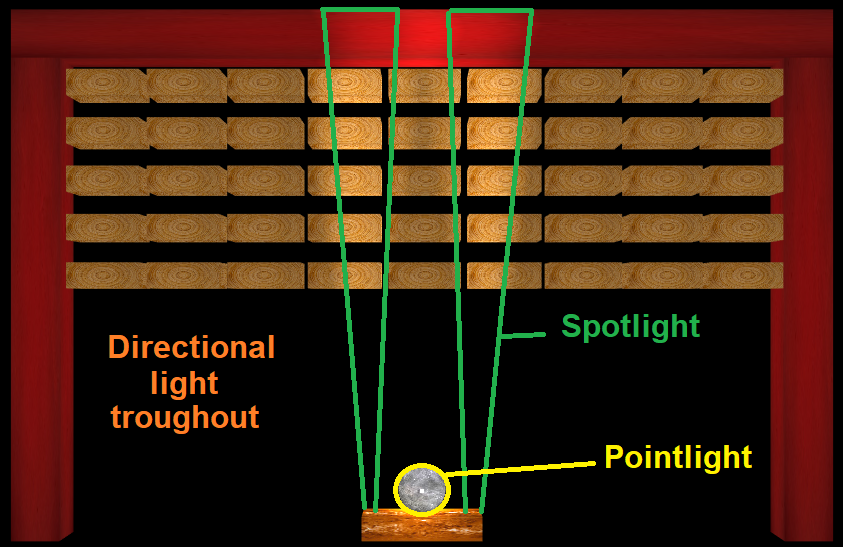
\includegraphics[width=\textwidth]{Images/Lights.png}
	\caption{Lights within the game}
\end{figure}